\documentclass[11pt,a4paper]{article}

% ---------- Packages ----------
\usepackage[a4paper,top=0.75in,bottom=0.70in,left=0.85in,right=0.85in]{geometry}
\IfFileExists{newtxtext.sty}{\usepackage{newtxtext,newtxmath}}{\usepackage{mathptmx}}
\usepackage{graphicx}
\usepackage{array}
\usepackage{booktabs}
\usepackage{enumitem}
\usepackage{titlesec}
\usepackage{fancyhdr}
\usepackage{setspace}
\usepackage{ragged2e}
\usepackage[hidelinks]{hyperref}
\usepackage{caption}
\usepackage{float}
\usepackage{tabularx}
\usepackage{longtable}
\usepackage{xcolor}
\usepackage{amsmath}
\sloppy
\usepackage[T1]{fontenc}
\usepackage{tikz}
\usetikzlibrary{arrows.meta,positioning,shapes.geometric,shapes.multipart,fit,calc,backgrounds}

% ---------- General formatting ----------
\setlength{\parindent}{0pt}
\setlength{\parskip}{4pt}
\setstretch{1.0}
\setlist[itemize]{leftmargin=0.28in,itemsep=1pt,topsep=1pt}
\setlist[enumerate]{leftmargin=0.30in,itemsep=1pt,topsep=1pt}
\AtBeginDocument{\fontsize{10.5}{12.0}\selectfont}

\titleformat{\section}
  {\normalfont\fontsize{16}{19}\selectfont}
  {}{0pt}{}
\titlespacing*{\section}{0pt}{4pt}{6pt}
\titleformat{\subsection}
  {\normalfont\fontsize{12.5}{15}\selectfont\bfseries}
  {}{0pt}{}
\titlespacing*{\subsection}{0pt}{5pt}{5pt}
\titleformat{\subsubsection}
  {\normalfont\fontsize{11.5}{14}\selectfont\bfseries}
  {}{0pt}{}
\titlespacing*{\subsubsection}{0pt}{4pt}{4pt}

\newcommand{\chaptertitle}[2]{%
  \vspace*{0pt}%
  {\normalfont\fontsize{22}{25}\selectfont #1\par}%
  \vspace{2pt}%
  \noindent\rule{\textwidth}{0.7pt}\par
  \vspace{7pt}%
  {\normalfont\fontsize{22}{25}\selectfont #2\par}
  \vspace{5pt}%
}

\captionsetup[figure]{font=small,labelfont=normal,textfont=it,justification=centering,skip=5pt}
\captionsetup[table]{font=small,labelfont=normal,textfont=it,justification=centering,skip=4pt}

\pagestyle{fancy}
\fancyhf{}
\renewcommand{\headrulewidth}{0pt}
\fancyfoot[C]{\small\thepage}

% Helpers
\newcommand{\tc}[1]{\texttt{\small #1}}
\newcommand{\toc}[3]{#1 #2 & \pageref{#3}\\}
\newcommand{\tocb}[3]{\textbf{#1 #2} & \textbf{\pageref{#3}}\\}

% ---------- TikZ styles ----------
\tikzset{
  >=Stealth,
  box/.style={draw,thick,rectangle,align=center,font=\footnotesize,inner sep=3pt,minimum height=0.55cm},
  tier/.style={draw,rectangle,dashed,inner sep=6pt,font=\scriptsize\itshape},
  uc/.style={draw,ellipse,align=center,font=\scriptsize,inner sep=1pt,minimum height=0.6cm},
  act/.style={draw,rectangle,rounded corners=4pt,align=center,font=\scriptsize,minimum height=0.55cm,inner sep=3pt,text width=3.6cm},
  dec/.style={draw,diamond,aspect=2.6,align=center,font=\scriptsize,inner sep=0pt},
  cls/.style={draw,rectangle split,rectangle split parts=2,font=\tiny,align=left,inner sep=2pt,text width=2.7cm},
  life/.style={densely dashed,gray},
  msg/.style={->,font=\tiny},
}

\begin{document}

% ============================================================
% COVER
% ============================================================
\thispagestyle{empty}
\vspace*{0.65in}
\begin{center}
{\fontsize{18}{22}\selectfont\bfseries UCS503P -- Software Engineering Project\par}
\vspace{0.22in}
{\fontsize{25}{30}\selectfont\bfseries ResQ: Crisis Coordination Platform for\\
Emergency Response\par}
\vspace{0.14in}
{\fontsize{14}{17}\selectfont A Real-Time Emergency Response and Dispatch Management System\par}

\vspace{0.45in}
{\fontsize{14}{17}\selectfont\bfseries FINAL EVALUATION REPORT\par}

\vspace{0.30in}
{\fontsize{12}{15}\selectfont
Submitted by:\par
\vspace{0.08in}
1024170226\quad Gurnoor Singh Marok\par
1024170043\quad Rishi Gupta\par
1027170237\quad Tamanna Chadha\par
1024170255\quad Kaif Ahmad\par
\vspace{0.08in}
Group: 3Q24 BE Third Year, CSE\par
\vspace{0.25in}
Submitted to:\par
Dr. Anushka\par
Final Evaluation, November 2026\par
Computer Science and Engineering Department\par
Thapar Institute of Engineering and Technology, Patiala\par
}
\vspace{0.3in}
{\small Live system: \href{https://swe-project-res-q.vercel.app}{swe-project-res-q.vercel.app}\quad|\quad
API health: \href{https://resq-backend-hx09.onrender.com/api/health}{resq-backend-hx09.onrender.com/api/health}\par}
\end{center}

\newpage

% ============================================================
% CONTENTS
% ============================================================
\thispagestyle{empty}
{\fontsize{22}{26}\selectfont Contents\par}
\vspace{8pt}

\begin{tabularx}{\textwidth}{@{}Xr@{}}
\tocb{1}{\quad Introduction}{ch1}
\toc{\quad 1.1}{\quad Background and Context}{s11}
\toc{\quad\quad 1.1.1}{\quad Problem Statement}{s111}
\toc{\quad 1.2}{\quad Project Objectives}{s12}
\toc{\quad 1.3}{\quad Progress Since the Mid-Semester Evaluation}{s13}
[2pt]
\tocb{2}{\quad Methodology and Design}{ch2}
\toc{\quad 2.1}{\quad System Architecture}{s21}
\toc{\quad\quad 2.1.1}{\quad High-Level Design}{s211}
\toc{\quad\quad 2.1.2}{\quad Technical Stack}{s212}
\toc{\quad\quad 2.1.3}{\quad Phased Development Methodology}{s213}
\toc{\quad 2.2}{\quad Domain Model and Database Design}{s22}
\toc{\quad 2.3}{\quad UML Diagrams}{s23}
\toc{\quad\quad 2.3.1}{\quad Use Case Diagram}{s231}
\toc{\quad\quad 2.3.2}{\quad Class Diagram}{s232}
\toc{\quad\quad 2.3.3}{\quad Request Lifecycle State Diagram}{s233}
\toc{\quad\quad 2.3.4}{\quad Sequence Diagram}{s234}
\toc{\quad\quad 2.3.5}{\quad Activity Diagram}{s235}
\toc{\quad 2.4}{\quad Implementation Details}{s24}
\toc{\quad\quad 2.4.1}{\quad Module 1: Lifecycle, Authorization and Concurrency}{s241}
\toc{\quad\quad 2.4.2}{\quad Module 2: Privacy and Coordinate Protection}{s242}
\toc{\quad\quad 2.4.3}{\quad Module 3: Real-Time Synchronization Layer}{s243}
\toc{\quad\quad 2.4.4}{\quad Module 4: Matching Engine and Verification}{s244}
\toc{\quad\quad 2.4.5}{\quad Module 5: Logistics, Inventory and Cancellation}{s245}
\toc{\quad\quad 2.4.6}{\quad Module 6: Messaging, Evidence and Notifications}{s246}
\toc{\quad\quad 2.4.7}{\quad Module 7: Analytics and Heuristic Classification}{s247}
\toc{\quad\quad 2.4.8}{\quad Module 8: User Interface and Design System}{s248}
\toc{\quad 2.5}{\quad Security Architecture and Role-Based Access Control}{s25}
[2pt]
\tocb{3}{\quad Deployment and Operations}{ch3}
\toc{\quad 3.1}{\quad Production Topology and Free-Tier Hosting}{s31}
\toc{\quad 3.2}{\quad Environment Configuration}{s32}
\toc{\quad 3.3}{\quad Seeded Demonstration Dataset}{s33}
\toc{\quad 3.4}{\quad Operational Runbook}{s34}
[2pt]
\tocb{4}{\quad Results and Evaluation}{ch4}
\toc{\quad 4.1}{\quad Testing Methodology}{s41}
\toc{\quad 4.2}{\quad Test Inventory}{s42}
\toc{\quad 4.3}{\quad Live Pilot Validation}{s43}
\toc{\quad 4.4}{\quad Security and Concurrency Verification}{s44}
\toc{\quad 4.5}{\quad Mobile and Cross-Viewport Audit}{s45}
\toc{\quad 4.6}{\quad Status of Proposal and Mid-Semester Targets}{s46}
\toc{\quad 4.7}{\quad Analysis}{s47}
[2pt]
\tocb{5}{\quad Conclusion}{ch5}
\toc{\quad 5.1}{\quad Summary of Work}{s51}
\toc{\quad 5.2}{\quad Key Findings and Lessons Learned}{s52}
\toc{\quad 5.3}{\quad Limitations}{s53}
\toc{\quad 5.4}{\quad Future Work and Recommendations}{s54}
\toc{\quad 5.5}{\quad Final Remarks}{s55}
[2pt]
\tocb{}{Appendix A: Demonstration Accounts and Script}{appA}
\tocb{}{Bibliography}{bib}
\end{tabularx}

\newpage

% ============================================================
% CHAPTER 1
% ============================================================
\label{ch1}
\chaptertitle{Chapter 1}{Introduction}

\subsection{1.1\quad Background and Context}\label{s11}

Emergency and disaster response is fundamentally a coordination problem before it is a technology problem. During a local emergency, the difficulty is rarely in collecting a report: a form and a map pin solve that initial part of the problem. The harder task is coordinating independent actors who hold partial information and different priorities, including affected people, volunteers, non-governmental organizations (NGOs), resource providers, and administrators.

Response capacity during a crisis is scarce. A request that receives duplicate attention while another remains unseen represents capacity that has not been used effectively. ResQ addresses this gap through a shared, auditable operational view of requests, responders, resources, locations, and status. It treats disaster response as an enforced state machine: every distress ticket carries a unique immutable code, is verified by an authorized dispatcher, is claimed under an exclusivity lock, and is closed only when the affected person confirms that help was received.

\subsubsection{1.1.1\quad Problem Statement}\label{s111}

Ad hoc approaches to local emergency coordination, such as phone calls, spreadsheets, messaging groups, and disconnected organizational dashboards, exhibit five recurring failure modes. The proposal named these FM-01 to FM-05, and each is mapped below to the mechanism the final system uses to resolve it.

\renewcommand{\arraystretch}{1.25}
\begin{tabularx}{\textwidth}{@{}p{0.5in}p{1.25in}p{1.8in}X@{}}
\toprule
\textbf{Code} & \textbf{Failure Mode} & \textbf{Real-World Breakdown} & \textbf{ResQ Solution}\\
\midrule
FM-01 & Duplicated or wasted effort & Several squads converge on one high-profile location while quieter pockets receive no aid & Atomic claim on verified requests; the losing responder receives HTTP 409 and the claim is broadcast in real time\\
FM-02 & Fragmented visibility & Information is trapped in private chats, spreadsheets and call logs & One synchronized map-and-rail console for all five roles, updated over Socket.IO\\
FM-03 & Unmatched partial supplies & A request for 100 blankets and 20 filters goes unserved because no single supplier can cover it & Itemized request manifests that several depots can fulfil partially until the quota is met\\
FM-04 & Absence of accountability & Calls are forwarded without confirmation; no audit trail of completed relief & Forward-only five-stage lifecycle; closure requires the affected person's confirmation; immutable status history\\
FM-05 & Location and contact exposure & Public posting of phone numbers and exact GPS exposes families to extortion and looting & Dual-tier privacy: fuzzed public coordinates and redacted contacts; precise data only for the verified claimant and administrators\\
\bottomrule
\end{tabularx}
\renewcommand{\arraystretch}{1}

\subsection{1.2\quad Project Objectives}\label{s12}

The objectives set at the proposal stage, and all met in the final system, were:

\begin{enumerate}
\item Implement a server-enforced five-stage request lifecycle (Unverified, Verified, In Progress, Resolved, Closed) with role-based authorization at every transition.
\item Build a unified map-and-log dispatch console used by the five project roles from one codebase, with actions adapting to the logged-in role.
\item Protect affected-person location and contact privacy through coordinate fuzzing and authorization-aware response redaction, in both REST and real-time channels.
\item Provide real-time cross-dashboard propagation of state changes through a self-hosted WebSocket layer, with a measured latency far below the 2-second target.
\item Provide a deterministic rule-based matching engine and multi-supplier partial fulfilment of resource manifests.
\item Provide request-scoped messaging, evidence attachments, notifications and an administrator analytics dashboard computed from immutable transition logs.
\item Validate the system through automated unit, integration, concurrency and Playwright end-to-end tests, and through a live pilot measured against the proposal targets.
\item Deploy the complete system on a live production environment using only free-tier, free/open-source services.
\end{enumerate}

\subsection{1.3\quad Progress Since the Mid-Semester Evaluation}\label{s13}

At the mid-semester checkpoint, ResQ had a working core: data model, lifecycle, authorization, privacy-aware location handling, a shared console and public submission/tracking. Real-time propagation, matching, messaging, analytics, end-to-end testing, a pilot and deployment were explicitly listed as future work. Table~\ref{tab:delta} summarizes what was delivered between the two evaluations.

\renewcommand{\arraystretch}{1.25}
\begin{table}[H]
\centering
\begin{tabularx}{\textwidth}{@{}p{1.65in}p{1.7in}X@{}}
\toprule
\textbf{Area} & \textbf{At Mid-Semester} & \textbf{At Final Evaluation}\\
\midrule
Domain model & 2 collections (User, Request) & 13 collections (organizations, resources, inventory, assignments, manifests, verifications, notifications, messages, evidence, incidents, categories)\\
Real-time layer & Planned & Self-hosted Socket.IO with post-write broadcast and dual-layer privacy\\
Matching & Planned & Four-factor deterministic scoring engine\\
Logistics & Not started & Depot dashboard, reserve/release/allocate, multi-supplier fulfilment\\
Messaging and evidence & Planned & Request-scoped messages, notifications, GridFS evidence storage\\
Analytics and AI triage & Planned & KPI dashboard (24h / 7d / all time); offline-safe keyword classifier\\
Testing & Backend unit/integration tests; Playwright not performed & 126 backend tests across 21 files plus 7 Playwright E2E scenarios; mechanically verified test inventory\\
Pilot & Pending & Live pilot on 20 September 2026 with measured results\\
Deployment & Local only & Live on Vercel, Render and MongoDB Atlas M0 at \$0.00\\
\bottomrule
\end{tabularx}
\caption{Delivered scope: mid-semester versus final evaluation}\label{tab:delta}
\end{table}
\renewcommand{\arraystretch}{1}

\newpage

% ============================================================
% CHAPTER 2
% ============================================================
\label{ch2}
\chaptertitle{Chapter 2}{Methodology and Design}

\subsection{2.1\quad System Architecture}\label{s21}

\subsubsection{2.1.1\quad High-Level Design}\label{s211}

ResQ is a decoupled full-stack system. A React single-page application is served from Vercel's edge network and talks to a stateless Express REST API over HTTPS (JWT-authenticated) and to a Socket.IO server over WebSocket. The API is the only component that talks to MongoDB, which is the source of truth. Socket events are emitted \emph{after} successful database persistence, so if the socket layer drops, REST endpoints and page reloads always show ground truth.

\begin{figure}[H]
\centering
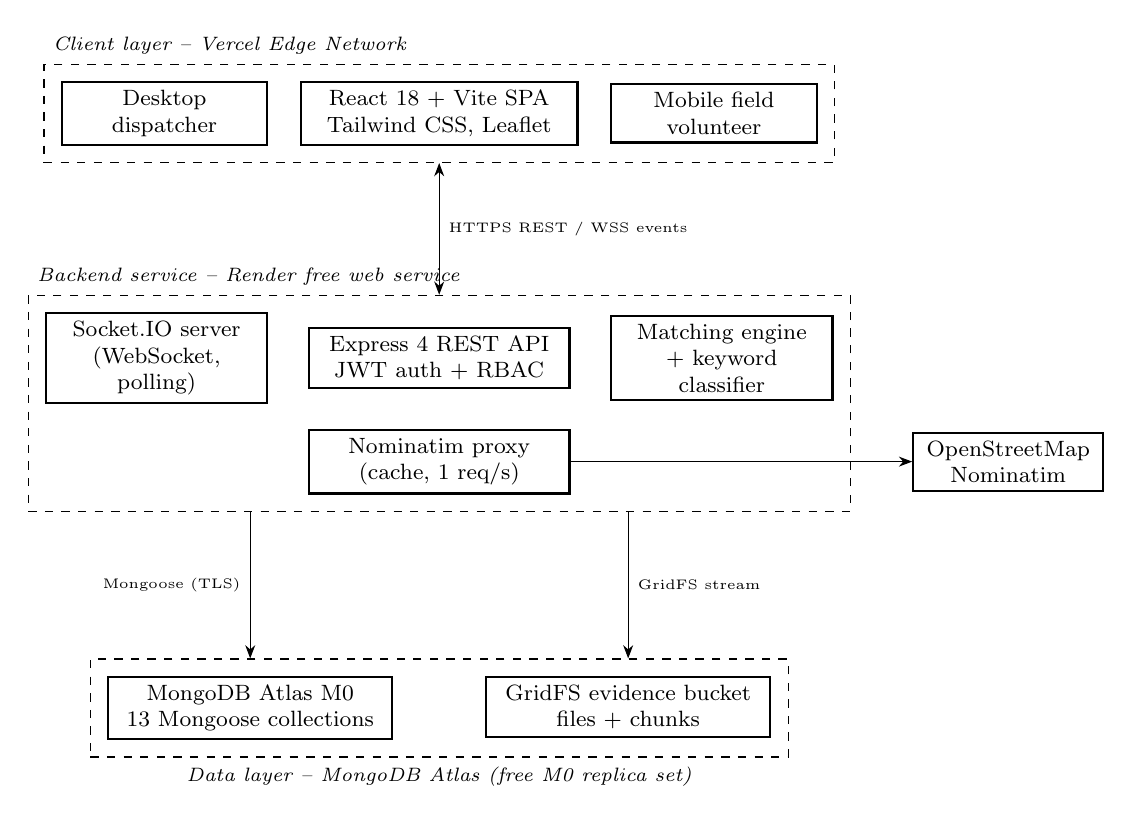
\begin{tikzpicture}[node distance=0.5cm]
\node[box,text width=3.3cm] (spa) {React 18 + Vite SPA\\Tailwind CSS, Leaflet};
\node[box,left=0.4cm of spa,text width=2.4cm] (desk) {Desktop dispatcher};
\node[box,right=0.4cm of spa,text width=2.4cm] (mob) {Mobile field volunteer};
\node[tier,fit=(desk)(spa)(mob),label={[font=\scriptsize\itshape,anchor=south west]north west:Client layer -- Vercel Edge Network}] (client) {};

\node[box,below=2.3cm of spa,text width=3.1cm] (api) {Express 4 REST API\\JWT auth + RBAC};
\node[box,left=0.5cm of api,text width=2.6cm] (sock) {Socket.IO server\\(WebSocket, polling)};
\node[box,right=0.5cm of api,text width=2.6cm] (match) {Matching engine\\+ keyword classifier};
\node[box,below=0.5cm of api,text width=3.1cm] (geo) {Nominatim proxy\\(cache, 1 req/s)};
\node[tier,fit=(sock)(api)(match)(geo),label={[font=\scriptsize\itshape,anchor=south west]north west:Backend service -- Render free web service}] (server) {};

\node[box,below=2.3cm of geo,xshift=-2.4cm,text width=3.4cm] (mongo) {MongoDB Atlas M0\\13 Mongoose collections};
\node[box,below=2.3cm of geo,xshift=2.4cm,text width=3.4cm] (grid) {GridFS evidence bucket\\files + chunks};
\node[tier,fit=(mongo)(grid),label={[font=\scriptsize\itshape,anchor=north]south:Data layer -- MongoDB Atlas (free M0 replica set)}] (data) {};

\node[box,text width=2.2cm] (osm) at ($(server.east |- geo)+(2.0,0)$) {OpenStreetMap\\Nominatim};

\draw[<->] (client.south) -- node[right,font=\tiny,fill=white]{HTTPS REST / WSS events} (server.north -| client.south);
\draw[->] (mongo |- server.south) -- node[left,font=\tiny,fill=white]{Mongoose (TLS)} (mongo.north |- data.north);
\draw[->] (grid |- server.south) -- node[right,font=\tiny,fill=white]{GridFS stream} (grid.north |- data.north);
\draw[->] (geo.east) -- (osm.west);
\end{tikzpicture}
\caption{Deployed ResQ architecture and topology}
\end{figure}

\subsubsection{2.1.2\quad Technical Stack}\label{s212}

The entire stack is free or open source, with no paid vendors and no credit-card gating.

\renewcommand{\arraystretch}{1.25}
\begin{tabularx}{\textwidth}{@{}p{1.15in}p{1.95in}X@{}}
\toprule
\textbf{Layer} & \textbf{Technology} & \textbf{Purpose / Constraint}\\
\midrule
Frontend & React 18, Vite, TypeScript, Tailwind CSS & Responsive SPA using design tokens from the Field Ops Ledger design system; no heavy UI library\\
Backend & Node.js 20+, Express 4, TypeScript & REST API, lifecycle, authorization, privacy redaction, 10 functional route domains\\
Database & MongoDB Atlas M0 + Mongoose & Persistent store for 13 collections; atomic conditional updates for claims\\
File storage & MongoDB GridFS & Evidence binaries survive Render's ephemeral container restarts; no S3/R2 cost\\
Authentication & Hand-rolled JWT + bcrypt (cost 10) & Stateless role-aware auth; \tc{requireAuth} and \tc{requireRole} guards\\
Real-time & Self-hosted Socket.IO 4.x & Attached to the Express HTTP listener; authenticated handshake; public and private rooms\\
Maps & react-leaflet + OpenStreetMap tiles & No API key, no billing liability\\
Geocoding & Nominatim via server proxy & In-memory cache, 1 req/s throttle, 400\,ms client debounce, strict User-Agent\\
Testing & Vitest, Supertest, Playwright & 126 backend tests (in-memory MongoDB) and 7 multi-context browser scenarios\\
Hosting & Vercel, Render, MongoDB Atlas & Edge SPA hosting, free web service, free M0 cluster\\
\bottomrule
\end{tabularx}
\renewcommand{\arraystretch}{1}

\subsubsection{2.1.3\quad Phased Development Methodology}\label{s213}

Development followed an incremental, milestone-based plan. Each phase left the system in a working, tested state, and Phase 2 explicitly preserved Phase~1 backward compatibility.

\renewcommand{\arraystretch}{1.2}
\begin{tabularx}{\textwidth}{@{}p{0.75in}p{1.85in}X@{}}
\toprule
\textbf{Phase} & \textbf{Theme} & \textbf{Main Deliverables}\\
\midrule
1 & Working prototype core & Ticket codes \tc{REQ-YYYY-NNNNNN}, JWT + bcrypt auth, five-stage lifecycle, Leaflet map with filterable dispatch rail, status-history audit trail\\
2 & Database and domain expansion & Growth from two to 13 collections without breaking Phase 1\\
2B & Logistics and management UIs & Depot dashboard, multi-provider partial fulfilment, incident management panel, organization roster\\
3 & Real-time layer & Socket.IO, post-write broadcast invariant, dual-layer real-time privacy\\
3B & Permission hardening & Security audit, \tc{requireRole} across all five roles with bidirectional 403/200 tests, cancellation lifecycle with stock release\\
4 & Matching and analytics & Four-factor scoring engine, analytics dashboard, optional keyword classifier\\
5 & E2E testing and pilot & Playwright multi-browser scenarios; live pilot of 20 September 2026\\
6 & Verified documentation & Mechanical test-inventory generator, final polish of the operations console\\
Deploy & Production release (19 Nov 2026) & Vercel + Render + Atlas, GridFS migration, seeded demo data, mobile audit\\
\bottomrule
\end{tabularx}
\renewcommand{\arraystretch}{1}

\subsection{2.2\quad Domain Model and Database Design}\label{s22}

The two-collection prototype (User and Request) was expanded into 13 Mongoose collections. Table~\ref{tab:collections} lists each with its role.

\renewcommand{\arraystretch}{1.2}
\begin{table}[H]
\centering
\begin{tabularx}{\textwidth}{@{}p{1.55in}X@{}}
\toprule
\textbf{Collection} & \textbf{Responsibility}\\
\midrule
User & Account, bcrypt hash, one of five roles, optional organization link\\
Request & Distress ticket: code, category, description, status, creator and claimant, precise and public coordinates, redacted contact, \tc{statusHistory}\\
Organization & Verified NGOs, relief agencies and logistics entities; responder rosters; depot identity\\
Resource & Standardized aid catalog (e.g., water, blankets, medical supplies)\\
ResourceInventory & Physical depot stock with available and reserved quantities\\
RequestResource & Itemized manifest lines on a request; supports split fulfilment by several suppliers\\
RequestAssignment & Explicit responder or depot deployment: lead responder, allocated quantities, state\\
Verification & Triage record: verifier, method (phone or field), priority, inspection notes\\
Notification & In-app event alerts per user\\
Message & Request-scoped discussion thread between requester and assigned responder\\
Evidence & Metadata of attachments; binaries are stored in GridFS (\tc{evidence.files}, \tc{evidence.chunks})\\
Incident & Declared major incident with a geographic radius; groups related requests\\
EmergencyCategory & Configurable categories with priority scores and default weights\\
\bottomrule
\end{tabularx}
\caption{The 13 domain collections}\label{tab:collections}
\end{table}
\renewcommand{\arraystretch}{1}

Indexing is dual: lookup indexes on request code, status and claimant, and geospatial fields for proximity queries. The deployed database uses about 1.8\,MB of the 512\,MB M0 allowance, so the storage limit is not a practical constraint for the project scope.

\newpage

% ============================================================
% UML
% ============================================================
\subsection{2.3\quad UML Diagrams}\label{s23}

The UML models below describe the final ResQ system. They extend the mid-semester models with the roles, entities and flows added in Phases 2 to 4.

\subsubsection{2.3.1\quad Use Case Diagram}\label{s231}

\begin{figure}[H]
\centering
\resizebox{\textwidth}{!}{%
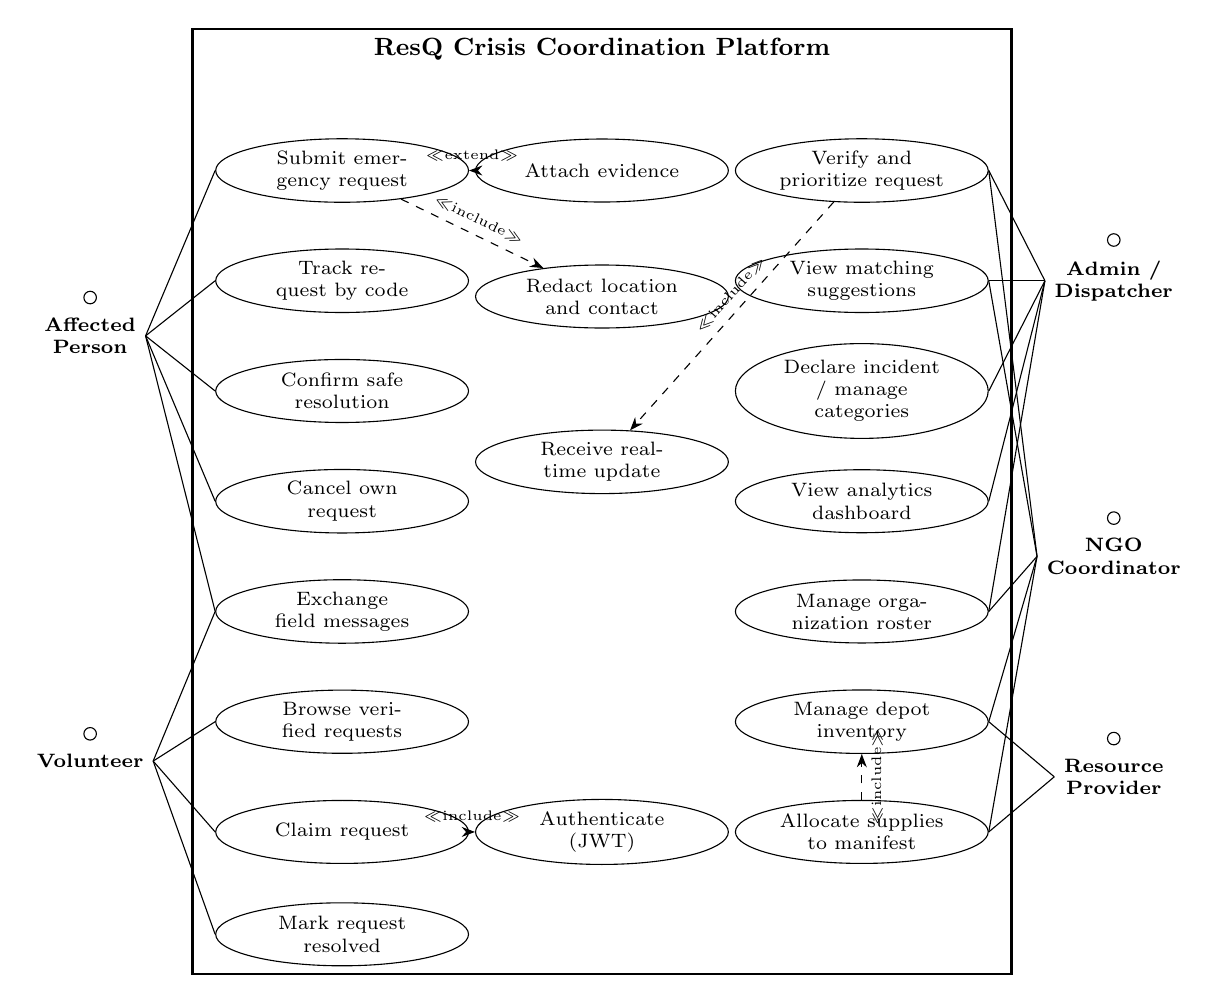
\begin{tikzpicture}[x=1cm,y=1cm,uc/.style={draw,ellipse,align=center,font=\scriptsize,inner sep=1pt,text width=2.2cm,minimum height=0.8cm}]
\draw[thick] (1.8,0.3) rectangle (12.2,-11.7);
\node[font=\small\bfseries,anchor=north] at (7.0,0.3) {ResQ Crisis Coordination Platform};
% left column
\node[uc] (u1) at (3.7,-1.5) {Submit emergency request};
\node[uc] (u2) at (3.7,-2.9) {Track request by code};
\node[uc] (u3) at (3.7,-4.3) {Confirm safe resolution};
\node[uc] (u4) at (3.7,-5.7) {Cancel own request};
\node[uc] (u5) at (3.7,-7.1) {Exchange field messages};
\node[uc] (u6) at (3.7,-8.5) {Browse verified requests};
\node[uc] (u7) at (3.7,-9.9) {Claim request};
\node[uc] (u8) at (3.7,-11.2) {Mark request resolved};
% middle column
\node[uc] (m1) at (7.0,-1.5) {Attach evidence};
\node[uc] (m2) at (7.0,-3.1) {Redact location and contact};
\node[uc] (m3) at (7.0,-5.2) {Receive real-time update};
\node[uc] (m4) at (7.0,-9.9) {Authenticate (JWT)};
% right column
\node[uc] (r1) at (10.3,-1.5) {Verify and prioritize request};
\node[uc] (r2) at (10.3,-2.9) {View matching suggestions};
\node[uc] (r3) at (10.3,-4.3) {Declare incident / manage categories};
\node[uc] (r4) at (10.3,-5.7) {View analytics dashboard};
\node[uc] (r5) at (10.3,-7.1) {Manage organization roster};
\node[uc] (r6) at (10.3,-8.5) {Manage depot inventory};
\node[uc] (r7) at (10.3,-9.9) {Allocate supplies to manifest};
% actors
\node[font=\scriptsize\bfseries,align=center] (A1) at (0.5,-3.6) {Affected\\Person};
\node[font=\scriptsize\bfseries,align=center] (A2) at (0.5,-9.0) {Volunteer};
\node[font=\scriptsize\bfseries,align=center] (A3) at (13.5,-2.9) {Admin /\\Dispatcher};
\node[font=\scriptsize\bfseries,align=center] (A4) at (13.5,-6.4) {NGO\\Coordinator};
\node[font=\scriptsize\bfseries,align=center] (A5) at (13.5,-9.2) {Resource\\Provider};
\foreach \a in {A1,A2,A3,A4,A5}{\node[draw,circle,inner sep=1.6pt,above=0.05cm of \a] {};}
% associations
\foreach \u in {u1,u2,u3,u4,u5}{\draw[thin] (A1.east) -- (\u.west);}
\foreach \u in {u5,u6,u7,u8}{\draw[thin] (A2.east) -- (\u.west);}
\foreach \u in {r1,r2,r3,r4,r5}{\draw[thin] (A3.west) -- (\u.east);}
\foreach \u in {r1,r2,r5,r6,r7}{\draw[thin] (A4.west) -- (\u.east);}
\foreach \u in {r6,r7}{\draw[thin] (A5.west) -- (\u.east);}
% include / extend
\draw[->,dashed] (u1) -- node[above,font=\tiny,sloped]{$\ll$include$\gg$} (m2);
\draw[->,dashed] (m1) -- node[above,font=\tiny]{$\ll$extend$\gg$} (u1);
\draw[->,dashed] (u7) -- node[above,font=\tiny]{$\ll$include$\gg$} (m4);
\draw[->,dashed] (r1) -- node[above,font=\tiny,sloped,pos=0.45]{$\ll$include$\gg$} (m3);
\draw[->,dashed] (r7) -- node[below,font=\tiny,sloped]{$\ll$include$\gg$} (r6);
\end{tikzpicture}}
\caption{ResQ use case diagram (five actors, \texttt{<<include>>} and \texttt{<<extend>>} relationships; NGO coordinators may also claim requests as lead unit)}
\end{figure}

\newpage

\subsubsection{2.3.2\quad Class Diagram}\label{s232}

\begin{figure}[H]
\centering
\resizebox{\textwidth}{!}{%
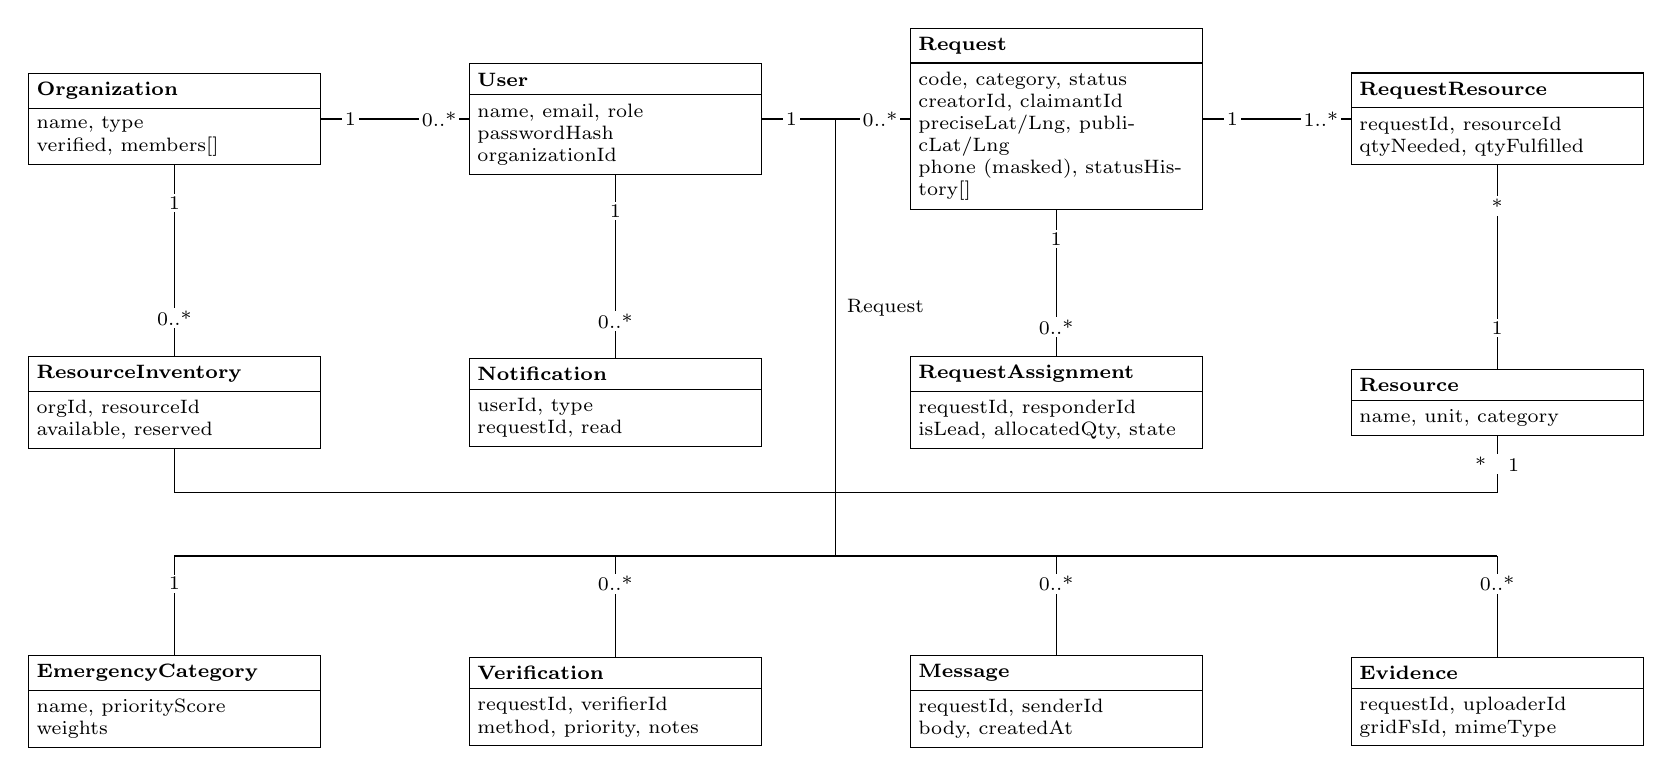
\begin{tikzpicture}[cls/.style={draw,rectangle split,rectangle split parts=2,font=\scriptsize,align=left,inner sep=3pt,text width=3.5cm,fill=white},ml/.style={font=\scriptsize,fill=white,inner sep=1pt}]
\node[cls] (org) at (0,0) {\textbf{Organization}\nodepart{second}name, type\\verified, members[]};
\node[cls] (user) at (5.6,0) {\textbf{User}\nodepart{second}name, email, role\\passwordHash\\organizationId};
\node[cls] (req) at (11.2,0) {\textbf{Request}\nodepart{second}code, category, status\\creatorId, claimantId\\preciseLat/Lng, publicLat/Lng\\phone (masked), statusHistory[]};
\node[cls] (rr) at (16.8,0) {\textbf{RequestResource}\nodepart{second}requestId, resourceId\\qtyNeeded, qtyFulfilled};
\node[cls] (inv) at (0,-3.6) {\textbf{ResourceInventory}\nodepart{second}orgId, resourceId\\available, reserved};
\node[cls] (note) at (5.6,-3.6) {\textbf{Notification}\nodepart{second}userId, type\\requestId, read};
\node[cls] (asg) at (11.2,-3.6) {\textbf{RequestAssignment}\nodepart{second}requestId, responderId\\isLead, allocatedQty, state};
\node[cls] (res) at (16.8,-3.6) {\textbf{Resource}\nodepart{second}name, unit, category};
\node[cls] (cat) at (0,-7.4) {\textbf{EmergencyCategory}\nodepart{second}name, priorityScore\\weights};
\node[cls] (ver) at (5.6,-7.4) {\textbf{Verification}\nodepart{second}requestId, verifierId\\method, priority, notes};
\node[cls] (msg) at (11.2,-7.4) {\textbf{Message}\nodepart{second}requestId, senderId\\body, createdAt};
\node[cls] (ev) at (16.8,-7.4) {\textbf{Evidence}\nodepart{second}requestId, uploaderId\\gridFsId, mimeType};

\draw (org) -- node[ml,pos=0.2]{1} node[ml,pos=0.8]{0..*} (user);
\draw (user) -- node[ml,pos=0.2]{1} node[ml,pos=0.8]{0..*} (req);
\draw (req) -- node[ml,pos=0.2]{1} node[ml,pos=0.8]{1..*} (rr);
\draw (user) -- node[ml,pos=0.2]{1} node[ml,pos=0.8]{0..*} (note);
\draw (req) -- node[ml,pos=0.2]{1} node[ml,pos=0.8]{0..*} (asg);
\draw (rr) -- node[ml,pos=0.2]{*} node[ml,pos=0.8]{1} (res);
\draw (org) -- node[ml,pos=0.2]{1} node[ml,pos=0.8]{0..*} (inv);
% inventory - resource route
\draw (inv.south) -- ++(0,-0.55) coordinate (r1) -- (r1 -| res.south) -- node[ml,pos=0.5]{*\quad 1} (res.south);
% request children bus
\coordinate (trunk) at ($(user.east)!0.5!(req.west)$);
\draw (trunk) -- (trunk |- 0,-5.55) coordinate (bus);
\draw (bus -| cat) -- (bus -| ev);
\foreach \c in {cat,ver,msg,ev}{\draw (bus -| \c) -- (\c.north);}
\node[ml,anchor=west] at ($(trunk)+(0.1,-2.4)$) {Request};
\node[ml] at ($(bus -| ver)+(0,-0.35)$) {0..*};
\node[ml] at ($(bus -| msg)+(0,-0.35)$) {0..*};
\node[ml] at ($(bus -| ev)+(0,-0.35)$) {0..*};
\node[ml] at ($(bus -| cat)+(0,-0.35)$) {1};
\end{tikzpicture}}
\caption{Simplified class diagram of the principal domain entities. Verification, Message, Evidence and the category reference attach to Request through \texttt{requestId}; Incident (name, centre, radius, \texttt{requestIds[]}) is omitted for clarity.}
\end{figure}

The Request class is the aggregate root: assignments, verifications, manifest lines, messages and evidence all reference a request by identifier. Inventory belongs to an organization (depot) and is reserved or released through allocation against manifest lines.

\subsubsection{2.3.3\quad Request Lifecycle State Diagram}\label{s233}

\begin{figure}[H]
\centering
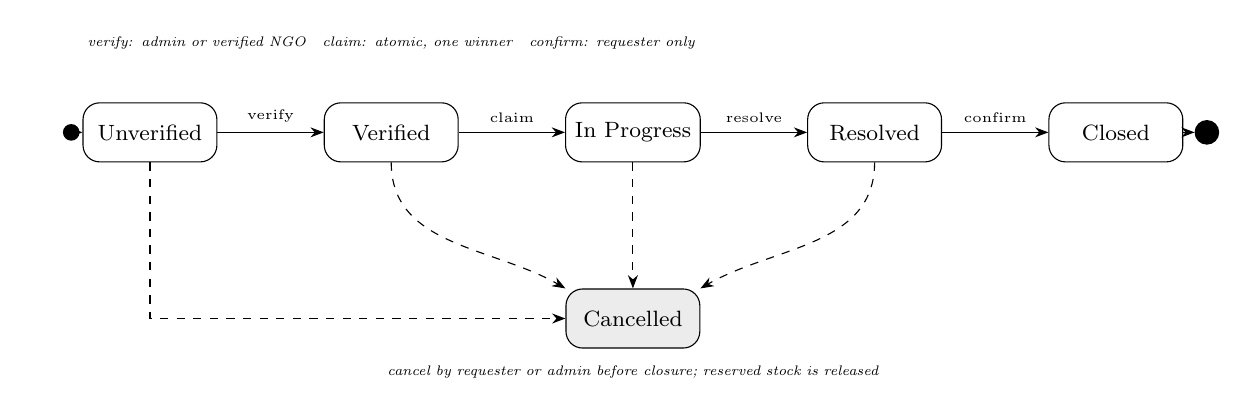
\begin{tikzpicture}[node distance=1.35cm,st/.style={draw,rounded corners=6pt,font=\footnotesize,minimum width=1.7cm,minimum height=0.75cm,align=center}]
\node[st] (s0) {Unverified};
\node[st,right=of s0] (s1) {Verified};
\node[st,right=of s1] (s2) {In Progress};
\node[st,right=of s2] (s3) {Resolved};
\node[st,right=of s3] (s4) {Closed};
\node[st,below=1.6cm of s2,fill=gray!15] (sc) {Cancelled};
\fill (-1.0,0) circle (3pt);
\draw[->] (-1.0,0) -- (s0);
\draw[->] (s0) -- node[above,font=\tiny]{verify} (s1);
\draw[->] (s1) -- node[above,font=\tiny]{claim} (s2);
\draw[->] (s2) -- node[above,font=\tiny]{resolve} (s3);
\draw[->] (s3) -- node[above,font=\tiny]{confirm} (s4);
\draw[->,dashed] (s0.south) |- (sc.west);
\draw[->,dashed] (s1.south) to[out=-90,in=150] (sc.north west);
\draw[->,dashed] (s2.south) -- (sc.north);
\draw[->,dashed] (s3.south) to[out=-90,in=30] (sc.north east);
\node[font=\tiny\itshape,below=0.1cm of sc,text width=8cm,align=center] {cancel by requester or admin before closure; reserved stock is released};
\draw[->] (s4) -- ++(1.0,0) node[draw,circle,fill=black,inner sep=3pt,right]{};
\node[font=\tiny\itshape,above=0.55cm of s1,text width=9cm,align=center] {verify: admin or verified NGO\quad claim: atomic, one winner\quad confirm: requester only};
\end{tikzpicture}
\caption{Forward-only five-stage lifecycle with cancellation branch}
\end{figure}

\newpage

\subsubsection{2.3.4\quad Sequence Diagram}\label{s234}

\begin{figure}[H]
\centering
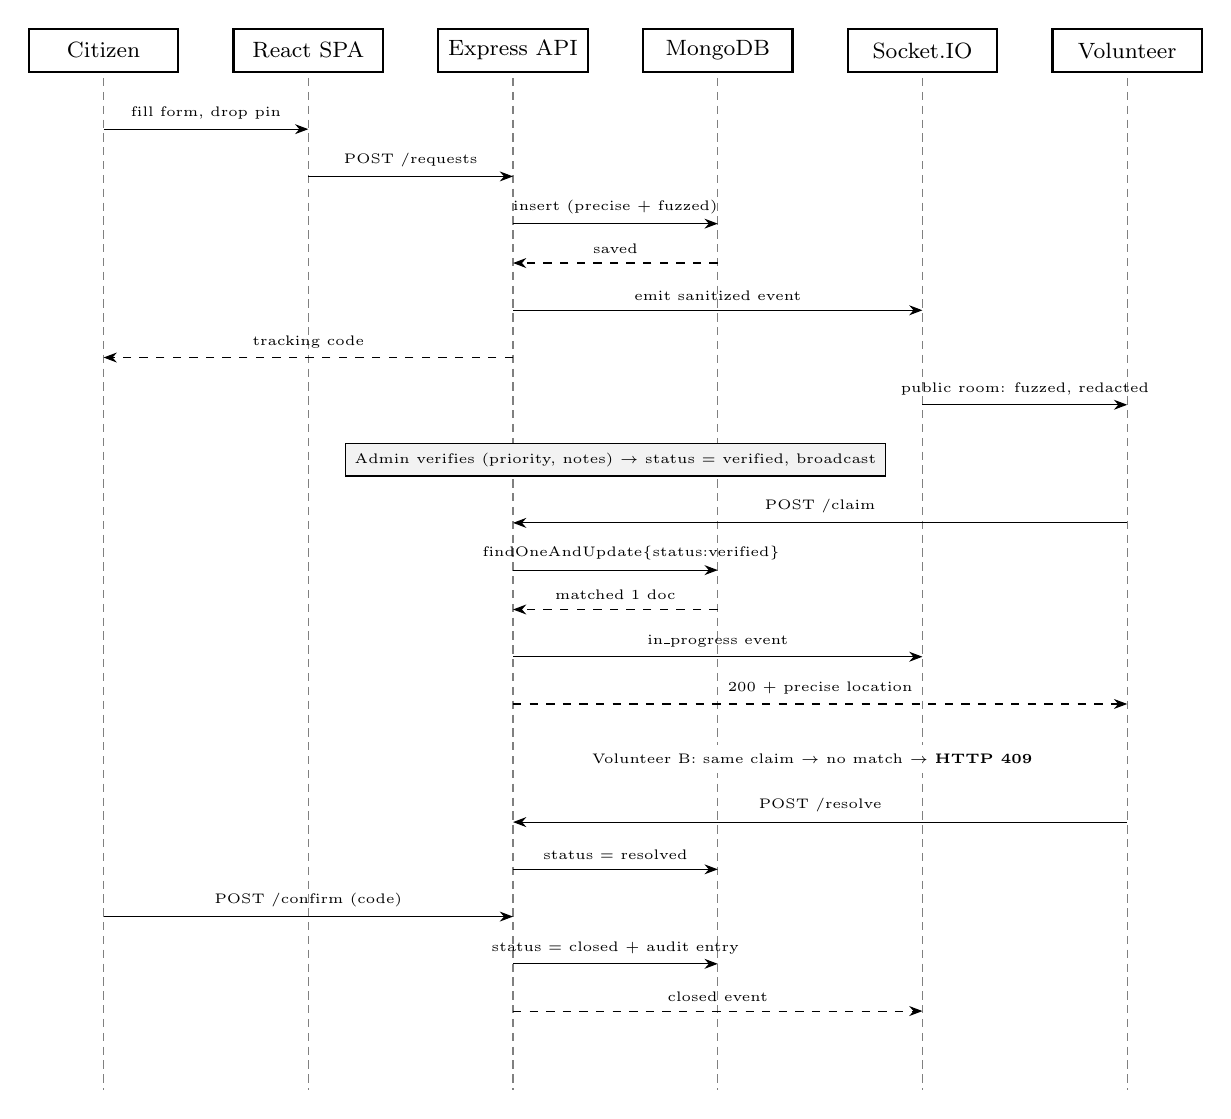
\begin{tikzpicture}[x=1cm,y=1cm]
\foreach \x/\n in {0/Citizen,2.6/{React SPA},5.2/{Express API},7.8/MongoDB,10.4/{Socket.IO},13.0/Volunteer}{
  \node[box,minimum width=1.9cm] at (\x,0) {\n};
  \draw[life] (\x,-0.35) -- (\x,-13.2);
}
\draw[msg] (0,-1.0) -- node[above,font=\tiny]{fill form, drop pin} (2.6,-1.0);
\draw[msg] (2.6,-1.6) -- node[above,font=\tiny]{POST /requests} (5.2,-1.6);
\draw[msg] (5.2,-2.2) -- node[above,font=\tiny]{insert (precise + fuzzed)} (7.8,-2.2);
\draw[msg,dashed] (7.8,-2.7) -- node[above,font=\tiny]{saved} (5.2,-2.7);
\draw[msg] (5.2,-3.3) -- node[above,font=\tiny]{emit sanitized event} (10.4,-3.3);
\draw[msg,dashed] (5.2,-3.9) -- node[above,font=\tiny]{tracking code} (0,-3.9);
\draw[msg] (10.4,-4.5) -- node[above,font=\tiny]{public room: fuzzed, redacted} (13.0,-4.5);

\node[draw,font=\tiny,fill=gray!10] at (6.5,-5.2) {Admin verifies (priority, notes) $\rightarrow$ status = verified, broadcast};

\draw[msg] (13.0,-6.0) -- node[above,font=\tiny]{POST /claim} (5.2,-6.0);
\draw[msg] (5.2,-6.6) -- node[above,font=\tiny,xshift=0.2cm]{findOneAndUpdate\{status:verified\}} (7.8,-6.6);
\draw[msg,dashed] (7.8,-7.1) -- node[above,font=\tiny]{matched 1 doc} (5.2,-7.1);
\draw[msg] (5.2,-7.7) -- node[above,font=\tiny]{in\_progress event} (10.4,-7.7);
\draw[msg,dashed] (5.2,-8.3) -- node[above,font=\tiny]{200 + precise location} (13.0,-8.3);
\node[font=\tiny,align=center,fill=white] at (9.0,-9.0) {Volunteer B: same claim $\rightarrow$ no match $\rightarrow$ \textbf{HTTP 409}};

\draw[msg] (13.0,-9.8) -- node[above,font=\tiny]{POST /resolve} (5.2,-9.8);
\draw[msg] (5.2,-10.4) -- node[above,font=\tiny]{status = resolved} (7.8,-10.4);
\draw[msg] (0,-11.0) -- node[above,font=\tiny]{POST /confirm (code)} (5.2,-11.0);
\draw[msg] (5.2,-11.6) -- node[above,font=\tiny]{status = closed + audit entry} (7.8,-11.6);
\draw[msg,dashed] (5.2,-12.2) -- node[above,font=\tiny]{closed event} (10.4,-12.2);
\end{tikzpicture}
\caption{Submission, verification, atomic claim (with 409 on conflict), resolution and confirmation}
\end{figure}

\newpage

\subsubsection{2.3.5\quad Activity Diagram}\label{s235}

\begin{figure}[H]
\centering
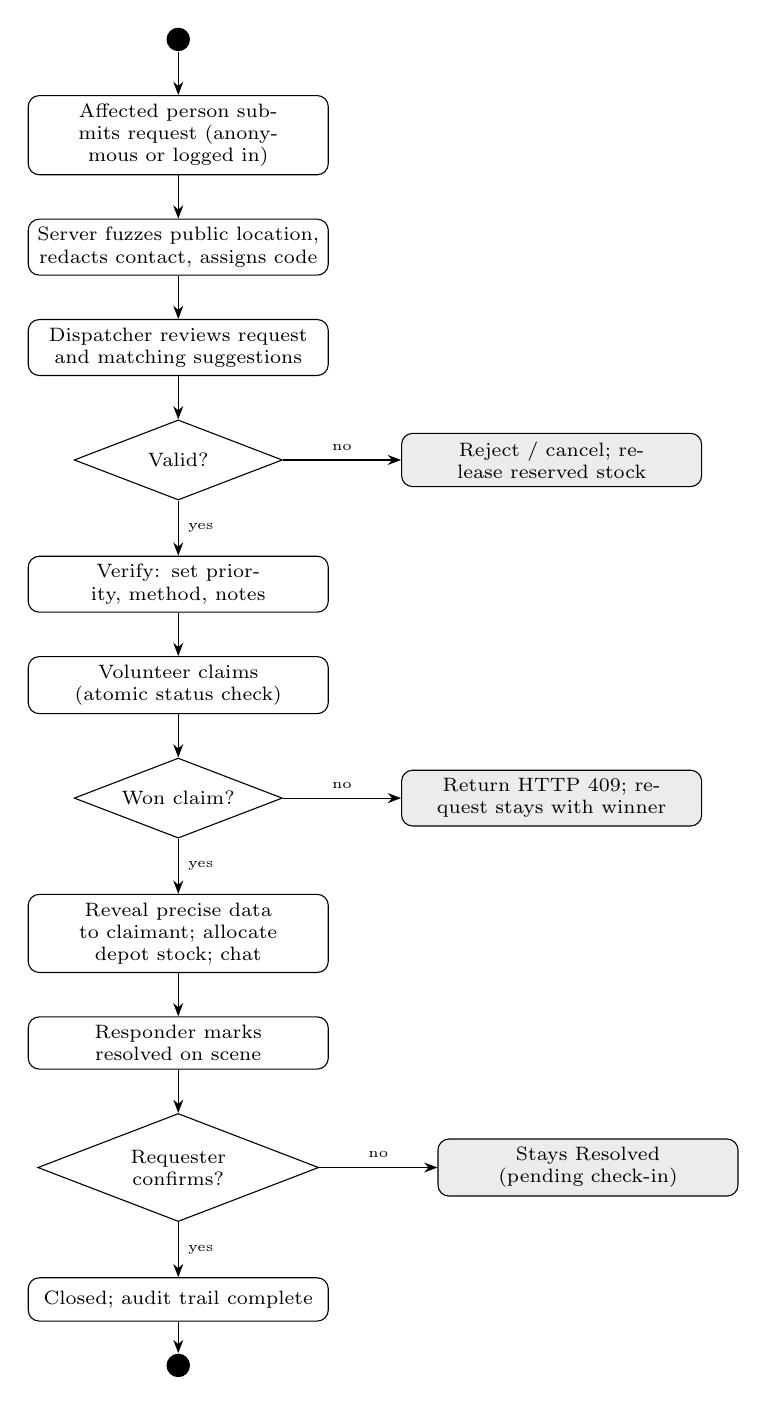
\begin{tikzpicture}[node distance=0.55cm]
\node[circle,fill=black,inner sep=3pt] (start) {};
\node[act,below=of start] (a1) {Affected person submits request (anonymous or logged in)};
\node[act,below=of a1] (a2) {Server fuzzes public location, redacts contact, assigns code};
\node[act,below=of a2] (a3) {Dispatcher reviews request and matching suggestions};
\node[dec,below=of a3,text width=2.2cm] (d1) {Valid?};
\node[act,right=1.5cm of d1,fill=gray!15] (rej) {Reject / cancel; release reserved stock};
\node[act,below=0.7cm of d1] (a4) {Verify: set priority, method, notes};
\node[act,below=of a4] (a5) {Volunteer claims (atomic status check)};
\node[dec,below=of a5,text width=2.2cm] (d2) {Won claim?};
\node[act,right=1.5cm of d2,fill=gray!15] (c409) {Return HTTP 409; request stays with winner};
\node[act,below=0.7cm of d2] (a6) {Reveal precise data to claimant; allocate depot stock; chat};
\node[act,below=of a6] (a7) {Responder marks resolved on scene};
\node[dec,below=of a7,text width=2.4cm] (d3) {Requester confirms?};
\node[act,right=1.5cm of d3,fill=gray!15] (pend) {Stays Resolved (pending check-in)};
\node[act,below=0.7cm of d3] (a8) {Closed; audit trail complete};
\node[circle,fill=black,inner sep=3pt,below=0.4cm of a8] (end) {};
\draw[->] (start)--(a1); \draw[->] (a1)--(a2); \draw[->] (a2)--(a3); \draw[->] (a3)--(d1);
\draw[->] (d1)--node[right,font=\tiny]{yes}(a4); \draw[->] (d1)--node[above,font=\tiny]{no}(rej);
\draw[->] (a4)--(a5); \draw[->] (a5)--(d2);
\draw[->] (d2)--node[right,font=\tiny]{yes}(a6); \draw[->] (d2)--node[above,font=\tiny]{no}(c409);
\draw[->] (a6)--(a7); \draw[->] (a7)--(d3);
\draw[->] (d3)--node[right,font=\tiny]{yes}(a8); \draw[->] (d3)--node[above,font=\tiny]{no}(pend);
\draw[->] (a8)--(end);
\end{tikzpicture}
\caption{Request fulfilment activity flow with authorization and state validation}
\end{figure}

\newpage

% ============================================================
% IMPLEMENTATION
% ============================================================
\subsection{2.4\quad Implementation Details}\label{s24}

\subsubsection{2.4.1\quad Module 1: Lifecycle, Authorization and Concurrency}\label{s241}

The lifecycle is centralized in transition logic. Each transition checks both the current state and the caller's authorization, preventing skipped or reversed states. Every transition appends a timestamped entry (actor, role, from, to) to the request's \tc{statusHistory}, which is treated as immutable: no role, including the administrator, may edit it. Closing a request requires confirmation by the original requester; the anonymous-request path uses the request code plus phone verification. Even an administrator cannot force-close a request, which preserves the accountability loop (FM-04).

Double-claiming is prevented at the database level instead of by application-level checks. The claim endpoint issues a single atomic conditional update:

\begin{center}
\tc{findOneAndUpdate(\{ \_id, status: 'verified' \}, \{ status: 'in\_progress', claimant \})}
\end{center}

If two volunteers claim simultaneously, MongoDB serializes the operations; the first matches the filter and the second matches nothing, which the API maps to \textbf{HTTP 409 Conflict}. This is verified both by concurrency tests and by a live two-browser demonstration.

\subsubsection{2.4.2\quad Module 2: Privacy and Coordinate Protection}\label{s242}

Location privacy is enforced structurally. Each request stores a precise coordinate pair and a separate public pair produced at submission by adding random jitter of up to roughly $\pm$500\,m:

\begin{center}
\tc{publicLat = preciseLat + (Math.random() - 0.5) * 0.009}
\end{center}

Public REST endpoints and public Socket.IO rooms emit only the public coordinates and replace phone numbers with ``REDACTED''. In the deployed build, public map and tracking feeds additionally round coordinates to two decimal places (about 1.1\,km) and redact names and phone numbers. Precise coordinates and direct contact details are released only to the verified claimant and to administrators. Because redaction is done at the API and socket boundary, hiding data in the frontend is never relied upon.

\subsubsection{2.4.3\quad Module 3: Real-Time Synchronization Layer}\label{s243}

Socket.IO is self-hosted on the same Express HTTP listener, so there is no third-party pub/sub cost. Three architectural rules govern it:

\begin{itemize}
\item \textbf{Post-write invariant:} events are emitted only after the database write succeeds, never before. REST remains the source of truth.
\item \textbf{Authenticated handshake:} connections with malformed or expired JWTs are rejected during the handshake.
\item \textbf{Dual-layer privacy:} the public room receives fuzzed, redacted payloads; precise payloads go only to the authenticated claimant's room.
\end{itemize}

\subsubsection{2.4.4\quad Module 4: Matching Engine and Verification}\label{s244}

The matching engine is deterministic and rule-based, with no model training or external service. It scores each candidate responder or depot against a pending request using four factors:

\[
\text{Score} = 0.35\times\text{Proximity} + 0.30\times\text{Suitability} + 0.20\times\text{Capacity} + 0.15\times\text{Availability}
\]

Proximity uses the Haversine great-circle distance; the skill matrix supplies suitability. Weights and category priority scores are configurable by administrators. The administrator console displays the ranked match readout so the human dispatcher stays in control: the engine advises and the dispatcher decides. Verification records capture the verifier, method (phone or field), priority level and inspection notes. NGOs may verify incoming tickets (if themselves verified) but cannot verify their own submitted requests.

\subsubsection{2.4.5\quad Module 5: Logistics, Inventory and Cancellation}\label{s245}

Depots maintain \emph{available} and \emph{reserved} balances per resource. A request may carry an itemized manifest, and several depots can contribute partial quantities until each line is fully served (FM-03). Reservation, release and allocation operations are guarded so that a quantity cannot be reserved beyond what is available. The cancellation lifecycle (``Option A'') lets a requester or administrator withdraw a ticket before closure and automatically releases any reserved stock back to the depots, so withdrawn requests never strand warehouse inventory.

\subsubsection{2.4.6\quad Module 6: Messaging, Evidence and Notifications}\label{s246}

Request-scoped message threads let the requester and assigned responders coordinate on scene, and in-app notifications alert users to verification, claim and message events. Evidence attachments were initially stored on local disk; because Render's free containers are ephemeral and wipe on restart, evidence was migrated to \textbf{MongoDB GridFS}. Files are chunked inside the Atlas cluster, survive server reboots and cost nothing extra.

\subsubsection{2.4.7\quad Module 7: Analytics and Heuristic Classification}\label{s247}

The administrator analytics dashboard computes Time-to-Match, propagation latency, double-booking conflict rate and confirmation rate directly from immutable transition logs, with 24-hour, 7-day and all-time filters. An optional keyword-based classifier suggests an emergency category from the request text. It runs on the server at zero cost, is never required for submission, and falls back gracefully when it has no confident result, giving complete offline resilience.

\subsubsection{2.4.8\quad Module 8: User Interface and Design System}\label{s248}

The frontend uses one shared map-and-rail console for all roles; only the available actions change. The ``Field Ops Ledger'' design system is built to reduce cognitive load under stress: high-contrast tabular lists, 1\,px hairline borders, Public Sans for civic authority and IBM Plex Mono for coordinates, timestamps and tracking IDs, with no gradients, soft shadows or pill badges. Dedicated dashboards cover the depot inventory, organization roster, incident management and analytics. The login page was cleaned for production: all demo shortcut cards and pre-filled credentials were removed, and an accessible Show/Hide password toggle with a 38\,px touch target was added. A calm loading banner explains the free-tier cold start to users.

\subsection{2.5\quad Security Architecture and Role-Based Access Control}\label{s25}

Defense in depth is applied at the route layer (Express middleware) and at the document layer (ownership checks). Passwords use bcrypt (cost 10); tokens are stateless JWTs signed with SHA-256 and carrying user ID and role claims; the signing secret is a 256-bit random string held only in the host's environment. Permissions were verified for all five roles with bidirectional tests: blocked roles receive HTTP 403 and permitted roles succeed.

\renewcommand{\arraystretch}{1.2}
\begin{table}[H]
\centering
\footnotesize
\begin{tabularx}{\textwidth}{@{}p{0.85in}XX@{}}
\toprule
\textbf{Role} & \textbf{Permitted} & \textbf{Rejected with 403}\\
\midrule
Affected person & Submit with or without login; track by code; message responder; confirm resolution; cancel own ticket & Claim, verify or prioritize; view others' precise location; manage inventory; analytics\\
\addlinespace
Volunteer & Browse verified tickets; claim; view precise location and phone after claim; message; mark resolved & Verify unverified reports; manage rosters; multi-supplier reservations; incidents or categories; analytics\\
\addlinespace
NGO & Manage organization profile; claim as lead unit; verify (if verified NGO); manage inventory; allocate supplies; query matching & Modify incidents; edit categories or weights; cross-theater analytics; self-verify own requests\\
\addlinespace
Resource provider & Catalog resources; maintain stock; reserve, release and allocate to manifests & Claim field tasks; verify requests; view victim contact details; declare incidents; analytics\\
\addlinespace
Admin & Verify with notes and priority; cancel any active ticket; manage categories, incidents, organizations and inventories; analytics & Bypass requester confirmation to falsify safe closure; alter immutable status history\\
\bottomrule
\end{tabularx}
\caption{Role-based access control matrix}
\end{table}
\renewcommand{\arraystretch}{1}

\newpage

% ============================================================
% CHAPTER 3
% ============================================================
\label{ch3}
\chaptertitle{Chapter 3}{Deployment and Operations}

\subsection{3.1\quad Production Topology and Free-Tier Hosting}\label{s31}

ResQ was deployed on 19 November 2026 and verified in live browser sessions across desktop and mobile viewports. The whole system runs on free tiers at a total cost of \$0.00 per month.

\renewcommand{\arraystretch}{1.2}
\begin{tabularx}{\textwidth}{@{}p{0.95in}p{1.0in}p{1.55in}X@{}}
\toprule
\textbf{Component} & \textbf{Platform} & \textbf{Plan} & \textbf{Limitation and Mitigation}\\
\midrule
Frontend & Vercel & Free Hobby, global edge & 100\,GB/month bandwidth, ample for demonstration; instant cache invalidation on git push\\
Backend & Render & Free web service, Node 20+ & Spins down after 15 min idle (about 35\,s cold start); mitigated by a pre-demo warm-up and an in-app loading banner\\
Database & MongoDB Atlas & M0 free replica set, MongoDB 8.0+ & 512\,MB limit; about 1.8\,MB used\\
Maps & OpenStreetMap & Public tile CDN & No key, no billing; bounded tile requests\\
Geocoding & Nominatim & Free API via server proxy & 1 req/s enforced by backend cache and 400\,ms client debounce\\
Files & MongoDB GridFS & Inside Atlas cluster & Survives Render's ephemeral file system\\
\bottomrule
\end{tabularx}
\renewcommand{\arraystretch}{1}

\subsection{3.2\quad Environment Configuration}\label{s32}

Secrets are held only in the hosting dashboards and are not committed to the repository.

\begin{itemize}
\item \textbf{Vercel (frontend):} \tc{VITE\_API\_URL} pointing to the Render backend; framework preset Vite; build command \tc{tsc \&\& vite build}; output directory \tc{dist}.
\item \textbf{Render (backend):} \tc{PORT=10000}, \tc{NODE\_ENV=production}, \tc{MONGODB\_URI} (Atlas SRV string), \tc{JWT\_SECRET} (256-bit random), and \tc{CORS\_ORIGIN} listing the Vercel origin and the local development origin.
\end{itemize}

A deployment issue worth recording: when a connection string omits an explicit database path, the driver may fall back to the default \tc{test} database. To remove this ambiguity, both the \tc{resq} and \tc{test} databases on Atlas were provisioned with identical collections, indexes and seeded records.

\subsection{3.3\quad Seeded Demonstration Dataset}\label{s33}

The production database is seeded with a geographically realistic flood scenario around Ludhiana and the Sutlej basin in Punjab, with one request at each lifecycle stage so every role can be demonstrated live.

\renewcommand{\arraystretch}{1.2}
\begin{tabularx}{\textwidth}{@{}p{1.35in}p{0.85in}X@{}}
\toprule
\textbf{Request} & \textbf{Stage} & \textbf{Scenario}\\
\midrule
\tc{REQ-2026-UNV-01} & Unverified & Basement flash-flood intrusion, Urban Estate Phase II, Ludhiana; ready for admin triage\\
\tc{REQ-2026-UNV-02} & Unverified & Insulin delivery needed, Civil Lines, Ludhiana\\
\tc{REQ-2026-VER-03} & Verified & Stranded family needing a rescue boat near Sutlej riverbank, Phillaur; ready for live claim demonstration\\
\tc{REQ-2026-INP-04} & In Progress & Elderly evacuation, Model Town; claimed by Responder A with active message thread\\
\tc{REQ-2026-RES-05} & Resolved & Drinking-water shortage, Sector 32A; supplies from Ludhiana Central Depot; awaiting citizen confirmation\\
\tc{REQ-2026-CLS-06} & Closed & Food-ration distribution, Gill Village; complete audit trail\\
\bottomrule
\end{tabularx}
\renewcommand{\arraystretch}{1}

Six accounts (admin, two volunteers, NGO coordinator, resource provider, affected citizen) are provisioned with bcrypt-hashed passwords; they are listed in Appendix~A.

\subsection{3.4\quad Operational Runbook}\label{s34}

\begin{enumerate}
\item \textbf{5--10 minutes before the demonstration:} request \tc{/api/health} and expect HTTP 200 with \tc{\{"status":"ok"\}}, then open the live frontend. This wakes the free-tier backend.
\item \textbf{Race-condition demonstration:} use a normal window for Responder A and an Incognito/Private window for Responder B so tokens are stored separately.
\item \textbf{Address search:} the Nominatim input is debounced at 400\,ms; pause briefly after typing to see suggestions.
\item \textbf{Cold start:} if the backend was idle for more than 15 minutes, the first request takes about 35\,s while the loading banner is shown.
\end{enumerate}

\newpage

% ============================================================
% CHAPTER 4
% ============================================================
\label{ch4}
\chaptertitle{Chapter 4}{Results and Evaluation}

\subsection{4.1\quad Testing Methodology}\label{s41}

\begin{itemize}
\item \textbf{Unit and integration testing:} Vitest and Supertest against an in-memory MongoDB cover scoring, utilities, models, REST endpoints and sockets.
\item \textbf{Concurrency testing:} simultaneous claims on the same request verify that exactly one succeeds and the other receives HTTP 409.
\item \textbf{Authorization testing:} each protected endpoint is tested in both directions (permitted role succeeds, forbidden roles receive 403).
\item \textbf{End-to-end testing:} Playwright runs seven multi-role scenarios using independent browser contexts, including real-time message exchange and isolation guarantees.
\item \textbf{Mechanical test inventory:} \tc{scripts/generate-test-inventory.ts} extracts every test block, cross-checks it against its annotation, and verifies line numbers and symbols in the code under test; it fails on any drift.
\item \textbf{Static analysis:} TypeScript strict typecheck (\tc{tsc --noEmit}) on frontend and backend.
\item \textbf{Live pilot and mobile audit:} a pilot on 20 September 2026 and a Playwright audit of the deployed system at mobile and desktop viewports.
\end{itemize}

\subsection{4.2\quad Test Inventory}\label{s42}

The final deployed backend suite (Vitest) runs \textbf{126 tests in 21 files, all passing, in 23.53\,s}, alongside \textbf{7 Playwright E2E scenarios} in Chromium. The mechanically verified inventory generated before deployment (2 November 2026) recorded 125 tests (17 unit, 101 integration, 7 E2E) with zero source discrepancies; its feature-area breakdown is shown in Table~\ref{tab:inventory}.

\renewcommand{\arraystretch}{1.1}
\begin{table}[H]
\centering
\footnotesize
\begin{tabularx}{\textwidth}{@{}Xrp{0.95in}X@{}}
\toprule
\textbf{Feature Area} & \textbf{Tests} & \textbf{Type} & \textbf{Components Under Test}\\
\midrule
Resources and inventory & 19 & Integration & routes/inventory.ts, routes/resources.ts\\
Authentication and roles & 15 & Unit / Int & middleware/auth.ts, routes/auth.ts\\
Request lifecycle & 12 & Integration & routes/requests.ts (claim, resolve, confirm)\\
Privacy and location & 11 & Unit / Int & utils/privacy.ts, routes/geocode.ts\\
Real-time (Socket.IO) & 10 & Integration & services/socket.ts, room broadcasts\\
AI classification & 8 & Unit / Int & services/classification.ts, offline fallback\\
End-to-end scenarios & 7 & Playwright & Multi-context workflows, comms isolation\\
Organizations & 6 & Integration & routes/organizations.ts\\
Verification & 6 & Integration & routes/requests.ts (verify endpoint)\\
Matching engine & 6 & Unit / Int & services/matching.ts (Haversine scoring)\\
Messaging and notifications & 6 & Integration & routes/notifications.ts, messages\\
Cancellation & 5 & Integration & routes/requests.ts (cancel, release stock)\\
Analytics & 5 & Integration & routes/analytics.ts (KPIs)\\
Categories and incidents & 3 & Integration & routes/categories.ts, routes/incidents.ts\\
Evidence attachments & 3 & Integration & routes/evidence.ts\\
Seed data and health & 3 & Unit / Int & routes/health.ts, scripts/seed.ts\\
\midrule
\textbf{Total (inventory)} & \textbf{125} & & 100\% passing\\
\bottomrule
\end{tabularx}
\caption{Feature-area distribution in the verified test inventory}\label{tab:inventory}
\end{table}
\renewcommand{\arraystretch}{1}

\subsection{4.3\quad Live Pilot Validation}\label{s43}

A live pilot was run on 20 September 2026. A single operator executed four concurrent emergency workflows (requests REQ-2026-382977, 535413, 123714 and 860087) across isolated browser sessions acting as citizen, dispatcher, volunteer and supplier. All metrics were computed from immutable database records and exported to \tc{pilot-results-2026-09-20.json}.

\renewcommand{\arraystretch}{1.3}
\begin{tabularx}{\textwidth}{@{}p{1.2in}p{1.25in}p{1.5in}X@{}}
\toprule
\textbf{Metric} & \textbf{Proposal Target} & \textbf{Measured} & \textbf{Outcome}\\
\midrule
Time-to-Match (triage to first claim) & Median $\leq$ 15 min & 1.0 min (min 1, max 1, n = 4) & Target met\\
Propagation latency (DB write to client render) & $<$ 2000\,ms (internal $<$ 500\,ms) & Median 23\,ms, p95 29\,ms (min 15, max 29, n = 8) & Target met\\
Double-booking rate & 0\% conflicts & 0 of 4 & Target met\\
Confirmation rate & No numeric target & 25\% (1 of 4 closed; 3 correctly pending check-in) & Benchmark only\\
\bottomrule
\end{tabularx}
\renewcommand{\arraystretch}{1}

The pilot also produced 4 assignments (all completed cleanly), 4 in-app notifications and 2 scoped two-way messages.

\textbf{Measurement condition.} As the evaluation protocol requires, the pilot was run by one operator on one machine, not by a dispersed field team. Values are reported as recorded, without filtering. The 1-minute Time-to-Match therefore reflects an ideal, co-located operator, and the 0\% double-booking result reflects a small sample of four tickets; the latter is reinforced by the dedicated concurrency tests in Section~4.4.

\subsection{4.4\quad Security and Concurrency Verification}\label{s44}

\begin{itemize}
\item \textbf{Concurrent claims:} when Responder A and Responder B claim the same verified request concurrently, A succeeds and B receives an explicit HTTP 409, verified in tests and live.
\item \textbf{Privacy:} public map and tracking feeds expose only fuzzed or rounded coordinates and redacted names and phones; precise data appears only for the verified claimant and administrators.
\item \textbf{Socket authentication:} malformed or expired tokens are rejected at the handshake.
\item \textbf{Production login:} no demo shortcuts, prefilled credentials or role auto-fill remain on \tc{/login}.
\item \textbf{Cancellation integrity:} cancelling a ticket releases reserved depot stock (5 tests).
\end{itemize}

\subsection{4.5\quad Mobile and Cross-Viewport Audit}\label{s45}

An automated Playwright audit of the deployed application at iPhone 14 (390$\times$844) and desktop (1440$\times$900) viewports confirmed layout stability, with no horizontal overflow on any screen.

\renewcommand{\arraystretch}{1.15}
\begin{tabularx}{\textwidth}{@{}p{1.9in}p{1.0in}p{0.85in}Xp{0.45in}@{}}
\toprule
\textbf{Screen} & \textbf{Viewport} & \textbf{Tap target} & \textbf{Touch / layout behavior} & \textbf{Result}\\
\midrule
Home (\tc{/}) & Mobile, desktop & $\geq$ 40\,px & No horizontal scroll & Pass\\
Submission form (\tc{/submit}) & Mobile & $\geq$ 42\,px & Pin drag and touch responsive & Pass\\
Tracking (\tc{/track/:id}) & Mobile & $\geq$ 38\,px & Zoom controls touch-enabled & Pass\\
Volunteer dashboard & Mobile & $\geq$ 40\,px & Dense list wraps cleanly & Pass\\
Depot and inventory & Mobile & $\geq$ 38\,px & Table scrolls inside container & Pass\\
Admin dispatch console & Mobile, desktop & $\geq$ 40\,px & Multi-pane stacks on mobile & Pass\\
Analytics dashboard & Mobile, desktop & $\geq$ 38\,px & Responsive grid cards & Pass\\
Login (\tc{/login}) & Mobile & $\geq$ 42\,px & Full-width inputs & Pass\\
\bottomrule
\end{tabularx}
\renewcommand{\arraystretch}{1}

\subsection{4.6\quad Status of Proposal and Mid-Semester Targets}\label{s46}

Table~\ref{tab:final} resolves every item that was ``pending'' or ``not yet applicable'' at the mid-semester evaluation.

\renewcommand{\arraystretch}{1.25}
\begin{table}[H]
\centering
\begin{tabularx}{\textwidth}{@{}p{1.5in}p{1.85in}X@{}}
\toprule
\textbf{Metric} & \textbf{Status at Mid-Semester} & \textbf{Status at Final Evaluation}\\
\midrule
Lifecycle transition correctness & Achieved (tests) & Achieved; also verified end-to-end in Playwright\\
Location and contact privacy & Achieved (tests) & Achieved; extended to Socket.IO rooms\\
Role-based authorization & Achieved (tests) & Achieved; bidirectional 403/200 tests for all five roles\\
Time-to-Match $\leq$ 15 min & Pending & Achieved: 1.0 min in pilot (single operator)\\
Cross-dashboard propagation $<$ 2 s & Not yet applicable & Achieved: median 23\,ms, p95 29\,ms\\
Double-booking rate 0\% & Not yet measurable & Achieved: 0/4 in pilot; atomic filter verified by concurrency tests\\
Free-tier stack & Maintained & Maintained: \$0.00 for all deployed services\\
Live demonstration & Future work & Live at swe-project-res-q.vercel.app\\
\bottomrule
\end{tabularx}
\caption{Final status of proposal and mid-semester targets}\label{tab:final}
\end{table}
\renewcommand{\arraystretch}{1}

\subsection{4.7\quad Analysis}\label{s47}

Three design decisions account for most of the results. First, pushing the double-booking guarantee into a single atomic MongoDB filter, rather than a read-then-write check in application code, makes the race condition impossible rather than merely unlikely. Second, broadcasting only after persistence kept the real-time layer simple and safe: a missed event never creates divergent state, and measured propagation of about 23\,ms is two orders of magnitude below the 2-second target. Third, performing redaction at the API and socket boundary meant that privacy needed to be verified in only one layer.

The mechanical test inventory deserves special mention as a quality practice: because documentation is generated from and checked against the source, the reported test figures cannot silently drift from the code.

\newpage

% ============================================================
% CHAPTER 5
% ============================================================
\label{ch5}
\chaptertitle{Chapter 5}{Conclusion}

\subsection{5.1\quad Summary of Work}\label{s51}

ResQ is now a complete, deployed, real-time crisis coordination platform. It provides a server-enforced five-stage lifecycle with an immutable audit trail, five-role RBAC, privacy-by-design location handling, a self-hosted real-time layer, a four-factor matching engine, multi-supplier logistics with cancellation and stock release, messaging, GridFS evidence storage, an analytics dashboard and an offline-safe heuristic classifier. It is validated by 126 backend tests, 7 Playwright scenarios, a live pilot and a mobile audit, and runs live on free tiers at \$0.00 per month.

\subsection{5.2\quad Key Findings and Lessons Learned}\label{s52}

\begin{itemize}
\item Concurrency control belongs in the database: an atomic conditional update eliminated double-booking without locks or queues.
\item Privacy must be enforced at the API and socket boundary; frontend hiding is not a security control.
\item Free-tier hosting has real operational constraints. Render's ephemeral disk forced the move from local-disk evidence to GridFS, the 15-minute idle spin-down required a warm-up protocol and loading banner, and a missing database path in the connection string required provisioning both the \tc{resq} and \tc{test} databases.
\item Rate-limited public services (Nominatim) need a server proxy, cache and client debounce to stay within usage policy.
\item Generated and mechanically verified documentation prevents drift between reports and code.
\item A shared console for all roles reduced duplicate UI code while keeping actions role-specific.
\end{itemize}

\subsection{5.3\quad Limitations}\label{s53}

\begin{itemize}
\item The pilot used a single operator on one machine with four requests; results demonstrate correctness under the tested workflow, not behaviour under large, dispersed, real-world load.
\item The matching engine is rule-based with fixed calibrated weights; it has not been tuned on real incident data.
\item The classifier is keyword-based and covers only the configured categories.
\item The Render free tier has a cold start of about 35\,s after idle, and Nominatim limits geocoding to 1 request per second.
\item The 512\,MB Atlas M0 limit and free-tier compute are adequate for the project scope but not for city-scale deployment.
\end{itemize}

\subsection{5.4\quad Future Work and Recommendations}\label{s54}

\begin{enumerate}
\item Run a multi-user field pilot with real volunteers and an NGO to measure Time-to-Match and confirmation rate in realistic conditions.
\item Load-test the real-time layer and migrate to a paid or self-managed tier with always-on compute before any real deployment.
\item Add offline-first behaviour (service worker and request queue) for areas with poor connectivity.
\item Add SMS or push notifications so users without the app open can be alerted.
\item Tune matching weights using recorded outcomes, and extend the classifier with a locally hosted model while keeping the offline fallback.
\item Add multilingual support (e.g., Punjabi and Hindi) and an accessibility review.
\item Commission an independent security assessment and add rate limiting and abuse detection for anonymous submissions.
\end{enumerate}

\subsection{5.5\quad Final Remarks}\label{s55}

The project set out to show that the coordination failures of emergency response can be addressed by a small number of enforced rules: one shared ledger, an atomic claim, a verified and confirmed lifecycle, and privacy at the boundary. The final system demonstrates each rule working in a live deployment, measured against the proposal targets, at no cost. The remaining work is mostly about scale and real-world validation rather than missing core capability.

\newpage

% ============================================================
% APPENDIX
% ============================================================
\label{appA}
\section*{Appendix A: Demonstration Accounts and Script}
\addcontentsline{toc}{section}{Appendix A}

Passwords for the demo accounts are supplied separately to evaluators and are intentionally not printed in this report.

\renewcommand{\arraystretch}{1.2}
\begin{tabularx}{\textwidth}{@{}p{1.15in}p{2.35in}p{0.8in}X@{}}
\toprule
\textbf{Persona} & \textbf{Email} & \textbf{Role} & \textbf{Verified Capabilities}\\
\midrule
System admin & admin.demo@resq.org & admin & Triage table, verification, matching readout, analytics\\
Volunteer A & responder.a@resq.org & volunteer & Claim, resolve, field messaging\\
Volunteer B & responder.b@resq.org & volunteer & Race-condition test: receives 409\\
NGO coordinator & coordinator.ngo@punjabrelief.org & NGO & Punjab Relief Network portal, team assignment\\
Resource provider & depot.logistics@ludhianadepot.org & provider & Ludhiana Central Emergency Depot inventory and allocation\\
Affected citizen & citizen.requester@example.org & citizen & Submit, track, confirm resolution\\
\bottomrule
\end{tabularx}
\renewcommand{\arraystretch}{1}

\subsection*{Suggested six-step live demonstration}
\begin{enumerate}
\item \textbf{Citizen} submits an emergency on \tc{/submit} and receives a tracking code.
\item \textbf{Admin} verifies it and reviews the matching scores.
\item \textbf{Concurrency race:} Responder A (normal window) and Responder B (private window) claim the same request; B receives 409.
\item \textbf{Depot} allocates resources while the responder and citizen chat.
\item \textbf{Responder} marks the request resolved; the \textbf{citizen} confirms and the ticket closes.
\item \textbf{Admin} reviews the analytics readout.
\end{enumerate}

\newpage

% ============================================================
% BIBLIOGRAPHY
% ============================================================
\label{bib}
\section*{Bibliography}
\addcontentsline{toc}{section}{Bibliography}

\begin{enumerate}[label={[}\arabic*{]},leftmargin=0.34in]
\item LaTeX Project Team. \textit{LaTeX2e: An updated version of LaTeX}. 2024.
\item Meta Open Source. \textit{React Documentation}. 2024.
\item OpenJS Foundation. \textit{Express -- Node.js web application framework}. 2024.
\item MongoDB, Inc. \textit{MongoDB Atlas and GridFS Documentation}. 2026.
\item Leaflet. \textit{Leaflet -- a JavaScript library for interactive maps}. 2024.
\item M. Jones, J. Bradley, N. Sakimura. \textit{JSON Web Token (JWT)}. RFC 7519, IETF, 2015.
\item Socket.IO. \textit{Socket.IO Documentation}. 2024.
\item Vitest. \textit{Vitest -- A Vite-native testing framework}. 2024.
\item Microsoft. \textit{Playwright -- Reliable end-to-end testing}. 2024.
\item OpenStreetMap Foundation. \textit{Nominatim Usage Policy}. 2024.
\item Vercel Inc. and Render Services Inc. \textit{Platform documentation and free-tier terms}. 2026.
\item OWASP Foundation. \textit{OWASP Top Ten}. 2024.
\end{enumerate}

\end{document}
